The following section is about the SmartAlvarTagDetection component. It is used for the scanning of the Alvar Tags on the MPS machines. The section explains how the component works, what the difficulties are and what changes have been made. 
 
\subsubsection{Overview}


This section is about the SmartAlvarTagDetection Component. The component is used to identify the Alvar Tags on the MPS machines, which is required for the exploration phase where the robots have to explore the game field and find MPS machines and identify the MPS based on their Alvar Tag. \\
Each MPS has their own Alvar Tag, one in the front and one in the back of the machine. This is important for the subsequent production phase. On the field there are seven machines for each team. There are four types of MPS Machines: Base station, Cap station, Ring station and Storage station. All together there are 14 machines with 28 unique Alvar Tags. \\

\begin{figure}[h]
\centering
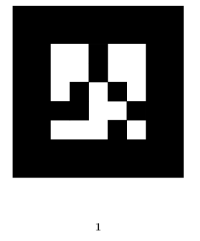
\includegraphics[scale=0.75]{pic/numberedMarker.png}
\caption{Shows an AlvarTag with corresponding ID}
\label{fig:smartAlvarFlow}
\end{figure}

The main idea is that the SmartAlvarTagDetection component identifies the tags. To do so, the component uses an algorithm to determine the Alvar Tag. Therefore, the component needs a picture of the Tag which is taken by a webcam mounted on each of the robotinos and operated by the SmartUnicapImageServer. The SmartAlvarTagDetection component is only one out of many components that are operated and instructed by the InstructionPlanner via the Sequencer (LISPServer). \\


\subsubsection{Previous State}

The team from the previous semester already had an implementation of the SmartAlvarTagDetection. In their version, they only had implemented the algorithm to scan pictures and identify whether there is a tag or not. They could not communicate with other components or the InstructionPlanner. \\

\begin{figure}[h]
\centering
\includegraphics[scale=0.5]{pic/SmartAlvarTagDetectionFlow.png}
\caption{Describes the flow of the SmartAlvarTagDetection Trigger Handler}
\label{fig:smartAlvarFlow}
\end{figure}


At first, the SmartUnicapImageServer is activated to take a picture and push an image to the SmartAlvarTagDetection. If the SmartUnicapImageServer is done, the LISP Server starts the SmartAlvarTagDetection Trigger Handler. The first thing the Trigger Handler does, is performing a validity check on the picture, to see if the picture can be used or not. If it is not valid, it returns a message saying that the image is not valid. But if it is valid, the image is converted into a greyscale picure, making it easier to recognize the Alvar Tags. Next, the marker detector, a method provided by the Alvar library, has to detect an Alvar Tag on the image. It determines the ID by scanning and detecting the tag. In a lookup table the detected ID is searched and if there is a tag belonging to the ID, then this marker is returned. Markers consist of the team colours, type of station and the side of the station. If the ID cannot be found, an error message is returned, otherwise a positive message is returned. \\

\begin {table}[h]
\caption{ID and MarkerDetectionState of MPS}
\label{tab:alvar_mps}
\begin{center}

 \begin{tabular}{|c | c|}
 \hline
 ID & MarkerDetectionState \\ [0.5ex] 
 \hline\hline
 1 & MARKER CYAN CAP STATION 1 FRONT \\ 
 \hline
 2 & MARKER CYAN CAP STATION 1 BACK \\
 \hline
 97 & MARKER MAGENTA CAP STATION 1 FRONT \\
 \hline
 98 & MARKER MAGENTA CAP STATION 1 BACK \\
 \hline
 193 & MARKER CYAN STORAGE STATION FRONT \\ [1ex] 
 \hline
 209 & MARKER MAGENTA STORAGE STATION FRONT \\ [1ex] 
 \hline
\end{tabular}
\end{center}
\end{table}

The main Problem in this approach was the weak error handling. When for instance no ID could be found on the image and therefore the lookup was not possible, then the entire Robotino crashed. Another problem was that there was no proper communication with the SmartRobotinoInstructionPlanner. When the MPS was detected and found in the lookup table, the positive message was directly sent to the RefBoxServer and not to the SmartRobotinoInstructionPlanner. The communication flow was not transparent. Another problem, not with the implementation but rather with the Alvar and OPENCV libraries, was that it only was possible to deploy the SmartAlvarTagDetection outo particular one computer, due to difficulties of installing the libraries.



\subsubsection{Current State}

The current version, which was used in the 2017 RoboCup German Open Logistics League in Magdeburg, is able to identify the tags, communicate with the InstructionPlanner via the LISP Server and has some sort of error handling. When the SmartAlvarTagDetection returns the message that no tag was found, the InstructionPlanner keeps triggering the component five times and if it still sends that no tag was found, one can be sure that there really is no tag and it is not a problem with the algorithm or bad picture quality. \\

\begin{figure}[h]
\centering
\includegraphics[scale=0.5]{pic/DeploymentAlvarTag.png}
\caption{Shows the model of the SmartAlvarTagDetection software component}
\label{fig:smartAlvarFlow}
\end{figure}



The current model of the SmartAlvarTagDetection software component consists of a SmartEventServer port, a SmartQueryClient port and a SmartParameterSlave port to communicate with other components. The SmartEventServer is connected to the LISP Servers' visualMarkerEventClient, which is used to trigger the SmartAlvarTagDetection Trigger Handler. The other is the SmartQueryClient which is connected to the SmartUnicapImageServers' imageQueryServer to request images that are taken by the webcam connected to the SmartAlvarTagDetection. A SmartParameterSlave can be used to change the parameters during runtime. The other noticeable thing is the SmartComponentParameter, which defines the behavior of the SmartAlvarTagDetection component to a Trigger behavior. The SmartEventTestHandler is used to check whether an event fires accordingly. In this case, it tests whether the correct MarkerDetectionState has been set. MarkerDetectionStates are the detected MPS as states. For instance, the tag with ID = 1 has been detected, then the MarkerDetectionState is set to MARKER CYAN CAP STATION 1 FRONT. Furthermore, a SmartComponentMetadata has to be added since it stores information about the version of the component\\

The component has been tested in isolation with the later described test deployment as well as in the master deployment. In the 2017 RoboCup German Open Logistics League contest, the SmartAlvarTagDetection component version in the master deployment was able to identify, determine and send the correct MPS to the Lisp Server. \\
The changes to the version of the previous semester include the communication flow with the Lisp Server, sending messages with the correct states and a more robust error handling. The component now handles different cases like, when a tag could not be found in the lookup table, when the image is not valid and when there is no marker on the image. Last year all these cases would have led to a dead lock in the robotino because these cases were not handled. Last semester the communication flow and the integration of the SmartAlvarTagDetection into the master deployment was intransparent. This has changed now, the component has a transparent way to communicate with and be triggered by the Lisp Server respectively by the SmartRobotinoInstructionPlanner. Another change was the portation of the Alvar and OPENCV libraries to the Ubuntu 16.04 version as well as the installation of the libraries on the student computers making it possible to deploy and use the SmartAlvarTagDetection on all student computers.

\subsubsection{Testing}

The SmartAlvarTagDetection component has its own test deployment DeployAlvarTest, where only the SmartAlvarTagDetection component is deployed on the Robotino. This is useful for testing only the SmartAlvarTagDetection component and opens the opportunity to increase the robustness of the component. \\

\begin{figure}[h]
\centering
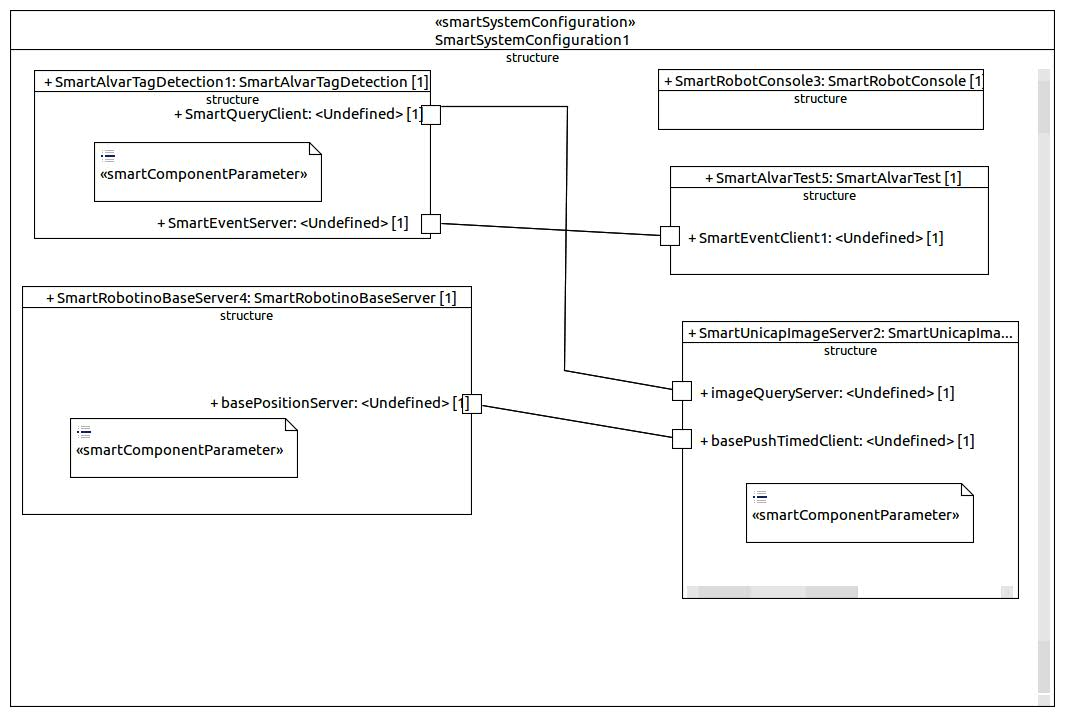
\includegraphics[scale=0.3]{pic/DeployAlvarTest.jpg}
\caption{Shows the test deployment of the SmartAlvarTagDetection component}
\label{fig:smartAlvarDeploy}
\end{figure}

The deployment consists of the SmartAlvarTagDetection component with the trigger handler to determine the tag, the SmartUnicapImageServer to provide the webcam picture, the SmartRobotConsole to set parameters of the robotino during runtime, the SmartRobotinoBaseServer to operate the robot and the SmartAlvarTest to see whether the correct event, the correct MarkerDetectionState, has been fired. The SmartRobotConsole is needed to activate and operate the SmartUnicapImageServer to push several images to the SmartAlvarTagDetection. The SmartAlvarTagDetection component needs to be triggered by the SmartRobotConsole, to do so the trigger parameter needs to be set manually. \\

The isolation tests were mostly about testing the detection of tags: in what angle does the robotino has to be towards the MPS and how far away can it be. As a result of the test cases, the angle should not be more than 45 or 120 degree to the orthogonal of the MPS and the farest point possible is about 6 metres away from the MPS. Within these settings the component could determine all tags correctly. Outside these settings, there occured problems that a tag was recognized but determined wrongly. Many times, the alvar tag was interpreted as a different alvar tag because the tags looked similiar and due to resolution of the robotinos' webcams the SmartAlvarTagDetection algorithm interpreted the tag wrongly.




